% easychair.tex,v 3.0 2011/10/24
%
% Select appropriate paper format in your document class as
% instructed by your conference organizers. Only withtimes
% and notimes can be used in proceedings created by EasyChair
%
% The available formats are 'letterpaper' and 'a4paper' with
% the former being the default if omitted as in the example
% below.
%
%\documentclass{easychair}
\documentclass[]{ciel}
%\documentclass[verbose]{easychair}
%\documentclass[notimes]{easychair}
%\documentclass[withtimes]{easychair}
%\documentclass[a4paper]{easychair}
%\documentclass[letterpaper]{easychair}
%\documentclass[notimes,custompaper,lmargin=1cm,rmargin=2cm,tmargin=.5cm,bmargin=1.5cm]{easychair}
%\documentclass[notimes,custompaper,lmargin=1cm,rmargin=2cm,tmargin=.5cm,bmargin=1.5cm]{easychair}

% This provides the \BibTeX macro
\usepackage{doc}
\usepackage{makeidx}

% In order to save space or manage large tables or figures in a
% landcape-like text, you can use the rotating and pdflscape
% packages. Uncomment the desired from the below.
%
% \usepackage{rotating}
% \usepackage{pdflscape}

% If you plan on including some algorithm specification, we recommend
% the below package. Read more details on the custom options of the
% package documentation.
%
% \usepackage{algorithm2e}

% Some of our commands for this guide.
%
\usepackage{xspace}
\usepackage{amssymb}
\usepackage{color}
\newcommand{\comment}[4]{\par\noindent\hspace*{-0.5cm}{\parbox{\columnwidth}{\textbf{\color{#1}//#2[#3]:#4}}}\par}

\newcommand{\easychair}{\textsf{easychair}}
\newcommand{\miktex}{MiK{\TeX}}
\newcommand{\texniccenter}{{\TeX}nicCenter}
\newcommand{\makefile}{\texttt{Makefile}}
\newcommand{\latexeditor}{LEd}
\newcommand{\ex}[1]{\emph{ex.}\xspace\emph{#1}}
\newcommand{\ie}[0]{\emph{c-à-d.}\xspace}
\newcommand{\mi}[1]{\comment{blue}{}{#1}{MI}}
\newcommand{\ch}[1]{\comment{green}{}{#1}{CH}}
\newcommand{\si}[1]{\comment{red}{}{#1}{SI}}
\newcommand{\FM}[0]{\textsc{fm}\xspace}
\newcommand{\Y}[0]{\textsc{YourCast}\xspace}
\newcommand{\LP}[0]{{ligne de produits}\xspace}
\newcommand{\LPS}[0]{{lignes de produits}\xspace}
\newcommand{\IR}[0]{interFMRelation}%\xspace}
\newcommand{\source}[0]{\textsc{source}\xspace}
\newcommand{\policy}[0]{\textsc{policy}\xspace}

%\makeindex

\usepackage{setspace}
\setstretch{0.94} 

%% Document
%%
\begin{document}

%% Front Matter
%%
% Regular title as in the article class.
%
\title{Vers la construction de workflows pour le filtrage sémantique de nouvelles}

% \titlerunning{} has to be set to either the main title or its shorter
% version for the running heads. Use {\sf} for highlighting your system
% name, application, or a tool.
%
\titlerunning{Vers la contruction de workflows...}

% For only the editors. Authors, please keep this commented out
% \volumeinfo
% 	{G. Sutcliffe, A. Voronkov}         % editors
% 	{2}                                 % number of editors
%	{{\easychair} 3.0 Beta 5, March 2011}      % event
%	{2}                                 % volume
%	{1}                                 % issue
%	{1}                                 % starting page number
%\indexededitor{Sutcliffe, Geoff}
%\indexededitor{Voronkov, Andrei}

%\headfootstyle
%	{}
%	{\sf}
%	{\footnotesize\sf}
%	{\small}

\volumeinfoECPS
	{CIEL Proceedings}
	{ECPS vol. 7999}

% Authors are joined by \and and their affiliations are on the
% subsequent lines separated by \\ just like the article class
% allows.
%
\author{
    Christophe Desclaux\\
    \affiliation{Université Nice Sophia Antipolis}\\
    \affiliation{\url{christophe@zouig.org}}\\
\and
    Simon Urli\\
    \affiliation{I3S, CNRS}\\
    \affiliation{Université Nice Sophia Antipolis}\\
    \affiliation{\url{urli@i3s.unice.fr}}\\
\and
    Mireille Blay-Fornarino\\
    \affiliation{I3S, CNRS}\\
    \affiliation{Université Nice Sophia Antipolis}\\
    \affiliation{\url{blay@polytech.unice.fr}}\\
\and
    Catherine Faron Zucker\\
    \affiliation{I3S, CNRS}\\
    \affiliation{Université Nice Sophia Antipolis}\\
    \affiliation{\url{faron@polytech.unice.fr}}\\
}

% \authorrunning{} has to be set for the shorter version of the authors' names;
% otherwise a warning will be rendered in the running heads.
%
\authorrunning{Desclaux, Urli, Blay-Fornarino and Faron Zucker}
\indexedauthor{Christophe, Desclaux}
\indexedauthor{Simon, Urli}
\indexedauthor{Mireille, Blay-Fornarino}
\indexedauthor{Catherine, Faron Zucker}

%%%%%%%%%%%%%%%%%%%%%%%%%%%%%%%%%%%%%%%%%%%%%%%%%%%
\maketitle
%%%%%%%%%%%%%%%%%%%%%%%%%%%%%%%%%%%%%%%%%%%%%%%%%%%
%------------------------------------------------------------------------------
% Abstract
%
\begin{abstract}
Le web se révèle aujourd'hui un merveilleux support de diffusion d'informations. Cependant, tandis que les sources se multiplient (flux rss, services web, ..), la quantité d'informations croît et il est nécessaire de les filtrer en fonction des centres d'intérêts des utilisateurs. Actuellement de nombreux outils qui exploitent les ontologies ou les thésaurus sont mis au point. Ils permettent d'annoter les informations, d'en déduire des critères et d'ensuite obtenir uniquement les informations pertinentes. La composition de ces outils constitue des workflows qui devraient encore s'enrichir grâce à l'apparition de nouvelles ontologies ciblées sur différents domaines et outils de lecture.  Cependant la construction de telles chaînes logicielles n'est pas à la portée de tous. \\
Dans cet article nous montrons comment de tels workflows ont été construits et présentons nos perspectives en matière de construction automatique de ces workflows en fonction des besoins utilisateur. Ce travail s'appuie sur le projet ANR Emergence \Y qui vise à automatiser la diffusion des informations sur de grands écrans, et pour lequel la pertinence des informations diffusées est donc particulièrement importante. 

\paragraph*{Mots-clés : }Web sémantique, Ligne de produits logiciels, Workflow, Modèle de variabilité
\end{abstract}

\begin{abstract}
Internet is becoming today a wonderful medium to broadcast informations. While sources are multiplying (RSS, Web Services, ...), the amount of informations is growing and it becomes necessary to filter them according to user interests. Many tools are currently developed that exploits ontologies or thesauri to annotate informations. They enable to query these annotations according to criteria to retrieve only the relevant informations. The composition of these tools constitute workflows that should be enriched by the emergence of new ontologies modeling different domains and text analysis tools. However the composition of these tools-chains is not accessible for everyone.\\
In this paper we show how these workflows are built and present our approach for automatically building workflows based on user needs. This work is supported by the ANR Emergence \Y project dedicated to automate the broadcasting of informations on large screens, and for which the relevance of informations published is important.

\paragraph*{Keywords: }Semantic Web, Software Product Line, Workflow, Feature Model
\end{abstract}

%------------------------------------------------------------------------------

\section{Introduction}
\label{sect:introduction}

Le web se révèle aujourd'hui un merveilleux support de diffusion d'informations. Tandis que les sources se multiplient (flux rss, services web, ..), la quantité des informations croît et il devient essentiel de les filtrer en fonction des centres d'intérêts des utilisateurs \cite{Bouzeghoub2005}. Des outils qui exploitent des ontologies ou des thésaurus ont été mis au point qui permettent d'annoter les informations, d'en déduire des critères et d'ensuite obtenir uniquement les informations pertinentes en formulant des requêtes sémantiques sur les annotations. 
Il est aujourd'hui possible de construire des workflows mettant en jeu ces différents outils pour d'une part annoter les flux d'informations et pour d'autre part sélectionner les informations pertinentes en fonction de la cible de diffusion. 

Cependant la construction de ces workflows reste technique malgré les nouveaux supports logiciels tels que les mashups \cite{Floyd2007,Milanovic2004}. En effet, elle se base sur de nombreux critères qui doivent être pris en compte pour assembler les services et le fait que ces services soient hétéroclites ne permet pas une génération aisée des applications. 
De plus de nouvelles ontologies, sources, systèmes d'annotations apparaissent régulièrement tandis que le web se démocratise \cite{Anderruthy2007,Bross2010}, ce qui occasionne des mises à jour régulières de ces workflows.

Dans ce contexte, nous décrivons dans cet article la construction de ces workflows, puis discutons leur production automatique  à partir d'un ensemble de caractéristiques sélectionnées par l'utilisateur au travers d'une approche basée sur les lignes de produits logiciels. 

Ce travail s'inscrit dans le cadre du projet ANR Emergence \Y\footnote{\url{http://yourcast.unice.fr}} qui vise à automatiser la diffusion des informations sur de grands écrans. Nous présentons ce contexte en section \ref{sect:introduction}.
Nous montrons dans la section \ref{sect:miseEnOuvre} les choix d'architectures  que nous avons faits pour mettre en place les workflows adaptés au projet. Forts de cette expérience, nous proposons en section \ref{sect:perspectives} de produire de tels workflows en utilisant un développement dirigé par les modèles et des modèles de variabilité (\textit{feature models})\cite{Report1990}.  La section \ref{sect:conclusion} conclut cet article. 


%------------------------------------------------------------------------------

\section{Contexte et besoins exprimés dans le projet \Y}
\label{sect:exemple}
Dans le cadre du projet \Y, nous visons à diffuser sur de grands écrans des informations en provenance de différentes sources en particulier celles issues du web. Or de tels systèmes exigent une adhérence forte aux attentes des utilisateurs et l'adéquation des informations avec les centres d'intérêts des personnes est essentielle à l'acceptation de tels systèmes. 

Or de \textit{nombreuses sources d'information} sont aujourd'hui disponibles sous la forme de flux RSS. Ceux-ci sont généralement classés selon leurs thématiques générales (technologies, international, médical, ...). Une première étude nous a conduit à nous intéresser à une vingtaine de flux RSS sur divers sujets. 

La \textit{sélection des informations} dans ces sources multiples repose alors sur la mise en place de critères et leur composition. 
Ainsi  quelques critères de sélection sont  pré-établis par les fournisseurs de contenus.  Par exemple sur le site de news de Google\footnote{\url{http://news.google.fr}} l'internaute peut accéder à des nouvelles liées à l'économie ou bien des news locales. Cependant il ne peut pas récupérer les nouvelles économiques liées par exemple à la ville de Marseille ou plus largement à la région PACA. Dans notre exploitation des flux RSS nous souhaitons fournir un filtrage multi-critères permettant un tri fin des nouvelles pour par exemple récupérer les nouvelles économiques concernant la région PACA. 

Pour capturer ces critères il existe actuellement différents systèmes tels que le service \textsl{Google Reader}\footnote{\url{http://www.google.fr/reader/}} ou bien celui \textsl{rssLounge}\footnote{\url{http://rsslounge.aditu.de}}. Cependant ceux-ci ne proposent pas de regroupement des flux ni de filtrage multi-critères de ceux-ci. 

Les exigences du  projet \Y sont celles d'un système intuitif qui permet de capturer simplement les besoins utilisateur à la fois en terme de choix des sources d'informations et de critères de sélection.

Pour cela, nous avons choisi d'enrichir des flux d'information en nous basant sur l'extraction d'entités nommées \cite{Charton2011} présentes dans un grand nombre de bases de données RDF. Nous utilisons pour cela des systèmes d'extraction d'information et d'annotation sémantique qui permettent d'ajouter des liaisons vers les entités nommées spécifiques.


%------------------------------------------------------------------------------

\section{Annotation et filtrage sémantiques de flux RSS}
\label{sect:miseEnOuvre}
Afin de permettre une sélection plus adéquate des informations en fonction de leur pertinence sémantique nous avons mis au point deux types de workflows, dont la figure \ref{fig:WF} présente  l'architecture générale : un workflow d'annotation sémantique des nouvelles et un workflow de filtrage sémantique des nouvelles (encadré par des tirets). La division en deux workflows est essentielle car elle permet de faire travailler nos workflows de manière asynchrone.

\begin{figure}[htb!]
	\begin{centering}
	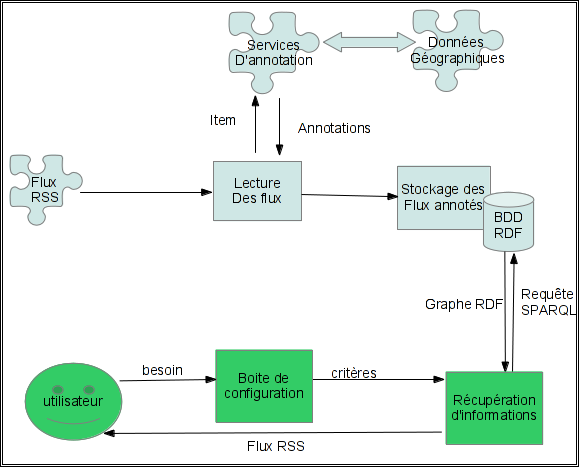
\includegraphics[width=0.9\textwidth]{diagramme-Archi.png}
	\caption{Workflows d'annotation et de filtrage sémantique de nouvelles}
	\label{fig:WF}
	\end{centering}
\end{figure}

\subsection{Workflow d'annotation sémantique des nouvelles}

\subsubsection{Lecture de flux RSS}
Le workflow se base sur la récupération périodique de flux RSS. Ces flux fournissent un lot des dernières nouvelles publiées par l'éditeur et sont mis à jour régulièrement.

\subsubsection{Annotation sémantique de nouvelles}
Des services enrichissent les nouvelles par des annotations et ces annotations elles-même peuvent être enrichies par l'utilisation de services de généralisation. 

Ainsi, nous utilisons des \textit{services d'annotation} pour qualifier chaque nouvelle par les entités nommées intéressantes la concernant. Les services d'annotation que nous avons utilisés sont : 
\begin{itemize}
	\item \textbf{OpenCalais}\footnote{http://www.opencalais.com} permet d'identifier dans le texte les entités correspondant à des lieux français ainsi que des noms de personnalités en langue anglaise. 
  \item \textbf{WikiMeta}\footnote{http://www.wikimeta.com} fonctionne sur le même principe qu'OpenCalais. Cependant le projet ne proposait pas au moment de nos recherches d'API permettant d'effectuer des requêtes et nous avons alors dû implémenter l'API Java se connectant à leurs services web. Elle permet de récupérer directement des entités nommées pointant vers la base de connaissances DBpedia ; il peut donc être utilisé seul en tant que service d'annotation sans utilisation d'un service de généralisation.
\end{itemize}

Nous faisons appel à des \textit{services de généralisation} qui travaillent en aval des services d'annotation pour ajouter des notions à une annotation :
\begin{itemize}
	\item \textbf{DBpedia}\footnote{http://dbpedia.org} travaille sur les données provenant du service d'annotation WikiMeta et permet de les enrichir sémantiquement à l'aide de liens vers d'autres ressources liées à l'élément.
  \item \textbf{INSEE geo}\footnote{\url{http://rdf.insee.fr/geo/}} La base de données RDF de l'INSEE permet de récupérer les ensembles géographiques liés à une entité nommée géographique. Ce service d'annotation géographique s'utilise donc uniquement en aval d'un service d'annotation classique qui récupère des informations géographiques. Il renvoie des URI vers les entités géographiques liées à la nouvelle étudiée. Nous utilisons pour cela une requête SPARQL.
\end{itemize}

\subsection{Workflow de filtrage des nouvelles}
Le workflow de filtrage permet de créer des critères utilisateurs afin de récupérer les données intéressantes sur la base des annotations. Notre workflow va dans un premier temps transformer les besoins utilisateurs en critères sous forme d'une liste de couples (TypeElement,entiteDescriptive). Ces couples sont ensuite envoyés à l'élément de connexion à la base de données qui effectue une requête SPARQL multi-critères sur la base de donnée RDF pour récupérer les nouvelles à fournir à l'utilisateur. Enfin le système génère un flux RSS personnalisé pour répondre aux besoins utilisateur et le fournit au client. Ce flux RSS va pouvoir être mémorisé par le client pour récupérer en temps réel les nouvelles informations.

\section{Vers la construction automatique de workflows }
\label{sect:perspectives}
Notre objectif à terme est de construire une ligne de produits qui capturerait les différentes sources et services disponibles, les qualifierait et permettrait à un utilisateur final de construire ses propres workflows d'annotation en le guidant dans sa sélection de différents services.

Du point de vue de l'utilisateur final, la construction automatique de workflows lui permettra, à partir d'un flux sélectionné, d'affiner la sélection des services d'annotations et généralisations qu'il souhaite utiliser afin d'obtenir une information enrichie par des annotations en fonction de ses besoins. 

A l'heure actuelle le workflow d'annotation interroge tous les services d'annotations disponibles, sans distinction de catégories, ce qui génère de nombreux appels de services dont la plupart sont inutiles. L'utilisation d'une construction automatique à partir des choix de l'utilisateur permettrait de restreindre les appels aux seuls services pertinents et donc d'accélérer les temps de traitements en réduisant la charge des services. 


\subsection{Lignes de produits de services}
Les choix que va faire l'utilisateur vont avoir un impact sur les trois concepts inhérents au workflow d'annotations représentés comme des pièces de puzzle dans la figure \ref{fig:WF} : les \textit{Flux d'information}, les \textit{Services d'Annotation} et les \textit{Services de Généralisation}. Chacun de ces concepts peut être vu comme une ligne de produits indépendante, à partir de laquelle l'utilisateur choisira le service qui lui convient. Nous représentons ces lignes de produits par des modèles de variabilité (\textsl{feature models}) notés FM \cite{Report1990}.

La figure \ref{fig:mmFM} montre le FM \textit{Service d'Annotation} qui permet de caractériser les services d'annotation existants (feature \textit{Produit}), les thèmes (feature \textit{Thème}) et les langues (Feature \textit{Langue}) supportés. La sélection d'une langue ou d'un thème influe directement sur le choix du service d'annotation par le jeu des contraintes internes au FM. On voit par exemple dans la figure \ref{fig:mmFM} que la sélection de la feature \textit{Santé} implique forcément la sélection du produit \textit{MetaMap}.

\begin{figure}[htb!]
	\begin{centering}
	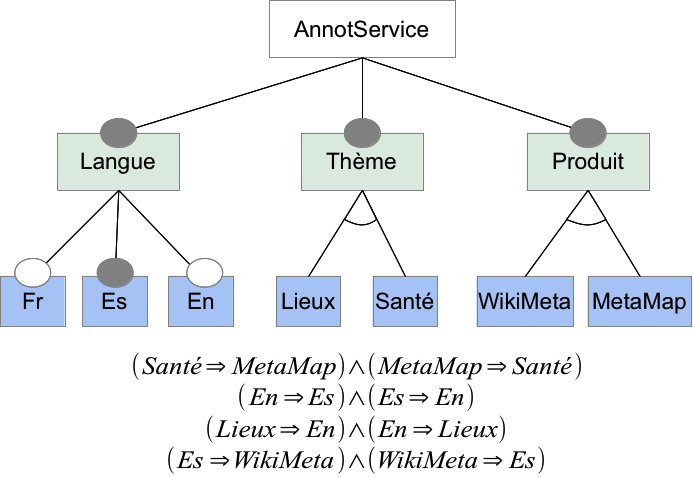
\includegraphics[scale=0.4]{FM.png}
	\caption{FM simplifié pour les services d'annotation}
	\label{fig:mmFM}
	\end{centering}
\end{figure}

L'utilisation du FM via un DSL ou des travaux des langages naturels n'ont pas encore été abordés dans nos travaux.
La construction du FM telle que présentée a été guidé par notre expérimentation. L'ajout de nouvelles sources devrait nous conduire à l'enrichir et éventuellement revoir sa structure.

\subsection{Modèle de mise en relation des Lignes de Produits Logiciels}
Notre but est de fournir un outil permettant à un utilisateur final de sélectionner des services cohérents en fonction de ses choix. Cela implique que certains choix de l'utilisateur dans un des FM ait un impact sur les autres FM.

Nous exprimons donc des relations entre les différents FM représentants les concepts du domaine. Une relation indique à la fois qu'un produit (i.e. un service) sera lié à un autre, mais aussi que sélectionner un produit influera sur la sélection d'un autre. En effet, les systèmes d'annotation sont spécialisés pour certains types d'informations, comme le service MetaMap\footnote{\url{http://metamap.nlm.nih.gov/}} spécialisé dans l'annotation de données médicales, et ne traitent que certaines langues.

Par exemple, un \textit{Flux} traitant de politique pourra être annoté par un ou plusieurs \textit{Services d'annotation} pouvant enrichir ce type d'information : les services, une fois sélectionnés, seront donc liés à ce flux, par exemple pour l'enrichir en données géographiques ou de santé. Cependant ce \textit{Flux} ne pourra pas être lié à un \textit{Service d'annotation} prenant en charge des langues différentes : la sélection du flux influe directement sur la sélection des \textit{Services d'annotation} à lier, tout simplement en empêchant l'utilisateur de sélectionner un service qui n'est pas compatible selon le critères de \textit{langue}.

Pour cela nous définissons et appliquons des opérations sur les FM \cite{Acher2011} afin de restreindre les choix de l'utilisateur, et ce en cascade. Pour reprendre notre exemple, la sélection d'un flux influe sur la sélection des annotations, en restreignant les services disponibles, ce qui aura également une influence sur les services de généralisation disponibles.

Sur la base du modèle ainsi obtenu qui fait référence aux différentes configurations, nous envisageons de générer automatiquement les workflows en utilisant à la fois les assets associés aux FM et les transformations sur les modèles.

%---------------------------------------------------------------
\section{Conclusion}
\label{sect:conclusion}
A l'heure où de plus en plus de services diffusent des flux d'informations sur le Web, il devient indispensable de posséder des outils afin de pouvoir filtrer ces informations. L'utilisation d'un système de filtrage sémantique par annotation des informations semble particulièrement intéressant en permettant à un utilisateur non-informaticien de définir de multiples critères de recherche et de filtrage.

Nous avons présenté dans cet article le système d'annotation ZeOntologyNewsExtractor\footnote{\url{https://github.com/descl/ZONE}} dont une preuve de concept est accessible sur \url{http://zone.zouig.org}. Nous avons explicité l'utilisation de l'ingénierie des connaissances pour enrichir sémantiquement des nouvelles. Puis nous avons présenté la nécessité de faire appel à l'ingénierie du logiciel et particulièrement la mise en place de workflows pour organiser les flux composant notre architecture. Enfin, nous avons présenté une amélioration possible de notre approche utilisant des lignes de produits logiciels afin de construire automatiquement nos workflows d'annotation.

L'intégration de ce travail au projet \Y constitue une validation  grande échelle du prototype. Ce projet a, en effet, pour objectif d'aider à la construction de systèmes de diffusion d'informations et il nous paraît intéressant d'être en mesure de proposer aux usagers un outil de filtrage sémantique d'information.

D'autre part des services tels que google ranking pourraient permettre de trier les informations par importance et l'utilisation de processus de regroupement permettrait de lier des news similaires entre elles \cite{Taddesse2010}.

%------------------------------------------------------------------------------
% Refs:
%

\label{sect:bib}
\bibliographystyle{plain}
\bibliography{christophe}

%------------------------------------------------------------------------------
\appendix

%------------------------------------------------------------------------------
% Index
%\printindex

%------------------------------------------------------------------------------
\end{document}

% EOF

